\documentclass[12pt, a4paper]{article}

% =============================================
% PAKETEAK
% =============================================
\usepackage[utf8]{inputenc}
\usepackage[T1]{fontenc}
\usepackage[basque]{babel}
\usepackage{geometry}
\usepackage{graphicx}
\usepackage{booktabs}
\usepackage{svg}
\usepackage{array}
\usepackage{float}
\usepackage{pifont}
\usepackage{hyperref}
\usepackage{xcolor}
\usepackage{amsmath}
\usepackage{amssymb}
\usepackage{fancyhdr}
\usepackage{parskip}
\usepackage{caption}
\usepackage{multirow}
\usepackage{longtable}
\usepackage{pgfplots}
\pgfplotsset{compat=1.18}

\geometry{top=2.5cm, bottom=2.5cm, left=3cm, right=3cm}

\hypersetup{colorlinks=true, linkcolor=black, citecolor=black, urlcolor=blue}

\pagestyle{fancy}
\fancyhf{}
\rhead{Spam Sailkatzailea -- MLP}
\lhead{Erabakiak Hartzeko Euskarri Sistemak}
\cfoot{\thepage}

% =============================================
% DOKUMENTUA
% =============================================
\begin{document}

% =============================================
% AZALA
% =============================================
\begin{titlepage}
    \centering
    \vspace*{1.5cm}
    {\Large \textbf{BILBOKO INGENIARITZA ESKOLA}}\\[0.3cm]
    {\normalsize Kudeaketaren eta Informazio Sistemen Informatikaren Ingeniaritzarako Gradua}\\[2cm]
    \rule{\textwidth}{1.5pt}\\[0.5cm]
    {\Huge \textbf{Spam Sailkatzailea}}\\[0.4cm]
    {\Large Multilayer Perceptron }\\[0.3cm]
    \rule{\textwidth}{1.5pt}\\[2cm]

    \begin{minipage}{0.45\textwidth}
        \textbf{Egileak:}\\
        Gorka Piedra\\
        Andoni Ortiz de Zarate\\
        Ibai Olaziregi\\
    \end{minipage}
    \begin{minipage}{0.45\textwidth}
        \raggedleft
        \textbf{Arloa:} Erabakiak Hartzeko Euskarri Sistemak\\[0.2cm]
        \textbf{Maila:} 3. maila\\
        \textbf{Lauhilabetea:} 2. lauhilabetea\\
    \end{minipage}
    \vfill
    {\large \today}
\end{titlepage}

% =============================================
% AURKIBIDEA
% =============================================
\tableofcontents
\newpage

% =============================================
% 1. TALDE-LANAREN ARDUREN BANAKETA
% =============================================
\section{Talde-lanaren arduren banaketa}

\begin{table}[H]
    \centering
    \caption{Taldekide bakoitzaren ardura eta inplementatutako zatiak}
    \begin{tabular}{p{2.5cm}p{4cm}p{6.5cm}}
        \toprule
        \textbf{Kidea} & \textbf{Ardura nagusia} & \textbf{Inplementatutako zatiak} \\
        \midrule
        Gorka Piedra &
        Dokumentazio teknikoa, kalitatearen ebaluazioa eta datuen prestaketa. &
        \textbullet{} JavaDoc dokumentazioaren sorrera proiektuko klase anitzetan. \newline
        \textbullet{} Datuak partitzeko logikaren inplementazioa (\texttt{DataSplit}). \newline
        \textbullet{} \texttt{GetModel.java} logika eredu entrenatuta lortzeko eta gordetzeko. \newline
        \textbullet{} \texttt{Evaluate.java} inplementazioa eredua ebaluatzeko. \newline
        \textbullet{} Erroreen kudeaketa eta \texttt{doku.tex} dokumentazioaren fintzea. \\
        \midrule
        Andoni Ortiz de Zarate &
        Esperimentazio azpiegitura eta analisia, entrenamendua eta ereduaren iraunkortasuna. &
        \textbullet{} MLP (\textit{Multilayer Perceptron}) garatzea eta doitzea \textit{grid search} bidez. \newline
        \textbullet{} Esperimentuen erregistroa kudeatzea   \texttt{ExperimentLogger.java} fitxategietan. \newline
        \textbullet{} Lortutako metriken analisia eta errepresentazioa grafikoen bidez.\newline 
        \textbullet{} Datuen hasierako karga eta ereduaren testeatzea. \\
        \midrule

        Ibai Olaziregi &
        Testuaren aurreprozesamendua, iragarpen-interfazea eta kodearen garbiketa. &
        \textbullet{} \texttt{EmailVectorizerAndSelector.java} garatzea bektorizaziorako eta atributu-hautapenerako. \newline
        \textbullet{} \texttt{Iragarri.java} inplementatzea mezu berrien iragarpenerako. \newline
        \textbullet{} Karaktere berezien tratamendua eta normalizazioa \texttt{TextNormalizer.java} fitxategian. \newline
        \textbullet{} Klase-diagramaren diseinua eta proiektuaren azken antolaketa (errefaktorizazioa eta garbiketa). \\
        \bottomrule
    \end{tabular}
    \label{tab:ardura}
\end{table}

Aipatzekoa da taldekide guztiok parte hartu dugula, neurri handiagoan edo txikiagoan, proiektuaren atal guztietan (hala nola dokumentazioan, kodearen garbiketetan edota testaketan). Hala ere, taulan agertzen den banaketak atal bakoitzean pisu handiena izan duen edo lan karga handiena bere gain hartu duen kidea islatzen du, ardura nagusiak argiago identifikatzeko asmoz.

\newpage
% =============================================
% 2. DATU-SORTAREN ANALISIA
% =============================================
\section{Datu-sortaren analisia}

\subsection{Datu gordinak}

Erabilitako datu-multzoa Enron-Spam corpusa da. Bi klasetan banatutako
mezu elektronikoz osatuta dago: \textbf{spam} (nahi ez dena) eta \textbf{ham} (legitimo).

Spam mezuak sustapen komertzialen, iruzurren eta premium zerbitzuen ingurukoak dira,
hizkera limurtzailea, maiuskulak, presazko estiloa eta estekak erabiliz
(adib.: \textit{``Free prize! Call now to claim your \pounds 1000''}).

Ham mezuak eguneroko komunikazio pertsonalak dira, hizkera informala,
laburdurak eta emotikonoak erabiliz (adib.: \textit{``Hey, what are you doing?''}).

\begin{table}[H]
    \centering
    \caption{Jatorrizko datu-multzoaren deskribapen kuantitatiboa (datu gordinak)}
    \begin{tabular}{lrrr}
        \toprule
        \textbf{Ezaugarria} & \textbf{Train} & \textbf{Dev} & \textbf{Test} \\
        \midrule
        Atributu nominalak  & 1     & 1     & 1     \\
        Atributu numerikoak & 0     & 0     & 0     \\
        String atributuak   & 1     & 1     & 1     \\
        Atributu guztira    & 2     & 2     & 2     \\
        \midrule
        Instantzia (spam $\oplus$)  & 1.200 & 150   & 150   \\
        Instantzia (ham $\ominus$)  & 2.937 & 368   & 367   \\
        Instantzia guztira          & 4.137 & 518   & 517   \\
        \bottomrule
    \end{tabular}
    \label{tab:datuak_gordinak}
\end{table}

Taula~\ref{tab:datuak_gordinak}-n ikusten den bezala, klaseen artean desoreka
nabarmena dago: spam instantziak ham instantzien \%29 baino ez dira.
Horrek eragina du ereduaren errendimenduan, bereziki spam klaseko recall-ean.

\subsection{Partiketa estratifikatua}

\texttt{DataSplit.java} fitxategiak \texttt{StratifiedRemoveFolds} metodoa erabiliz
datu-multzoa hiru azpimultzotan banatzen du, klaseen proportzioa mantenduz
partiketa guztietan. Partiketa \textbf{\%80/\%10/\%10} egin da:

\begin{itemize}
    \item \textbf{Train (\%80):} 4.137 instantzia -- eredua entrenatzeko
    \item \textbf{Dev (\%10):} 518 instantzia -- parametroak optimizatzeko
    \item \textbf{Test (\%10):} 517 instantzia -- azken iragarpenak egiteko
\end{itemize}

\newpage
% =============================================
% 3. AURREPROZESAMENDUA
% =============================================
\section{Aurreprozesamendua}

Sailkapen-eredu bat entrenatu aurretik, ezinbestekoa da datu gordinak (string formatukoak) garbitzea eta estandarizatzea. Posta elektronikoek (bereziki spam-ak) zarata handia izan ohi dute: HTML etiketak, estekak, karaktere bereziak eta informazio semantikorik gabeko hitzak. Atal honetan, aplikatutako garbiketa-prozesuak, horien helburua eta datuetan izandako eragin kuantitatiboa azaltzen dira.

\subsection{Datu gordinen garbiketa: Zer egin da eta zertarako?}
Lehenengo urratsean, gure \texttt{TextNormalizer.java} klaseak espresio erregularrak (Regex) erabiltzen ditu testu gordineko patroi espezifikoak ezagutu eta ordezkatzeko:

\begin{itemize}
    \item \textbf{URLak eta Estekak:} \textit{http://...} bezalako estekak \texttt{URL\_TOKEN} marka batekin ordezkatzen dira. Spam mezuetan oso ohikoa da estekak egotea, baina URL zehatzak berak ez du balio sailkapenerako, bere presentziak baizik.
    \item \textbf{Helbide elektronikoak:} Posta helbideak \texttt{EMAIL\_TOKEN} gisa etiketatzen dira, datu pertsonalen zarata murriztuz eta ereduak patroi orokorra ikas dezan.
    \item \textbf{HTML etiketak:} Etiketa guztiak ezabatzen dira, barruko testu garbia soilik mantenduz.
\end{itemize}

\subsection{Hizkuntza-tratamendua (NLP)}
Testua garbitu ondoren, zenbait eraldaketa linguistiko aplikatzen zaizkio testuari hitzak estandarizatzeko (geroago bektorizazio prozesuan erabiliko direnak):

\begin{itemize}
    \item \textbf{Minuskulizazioa:} Maiuskulak eta minuskulak berdintzen dira (\textit{``FREE''} eta \textit{``free''} token berdin gisa tratatzeko). Honek ereduaren sakabanaketa saihesten du.
    \item \textbf{Stopwords iragazkia (\texttt{Rainbow}):} Informazio semantiko esanguratsurik ez duten hitzak ezabatzen dira (artikuluak, preposizioak, adib.: \textit{``the''}, \textit{``is''}). Horrek zarata murrizten du.
    \item \textbf{Stemming (\texttt{LovinsStemmer}):} Hitzak beren erro lexikora murrizten dira (adib.: \textit{``running''} eta \textit{``runs''} $\rightarrow$ \textit{``run''}).
\end{itemize}

\subsection{Erabaki esperimentalen justifikazio kuantitatiboa}
Aurreko NLP teknikak (bereziki Stopwords eta Stemming) ez dira ausaz aukeratu. Iragazki bakoitza banan-banan ebaluatu beharrean, \textbf{aurreprozesamendu-bloke osoaren} (Normalizazioa + NLP) eragin bateratua neurtu da, ereduaren dimentsionalitatean eta kalitatean duen benetako inpaktua ikusteko.

Testu librea sailkatzean agertzen den arazo nagusietako bat dimentsionalitate altua da. Hurrengo taulan ikus daiteke zein den NLP garbiketa aplikatu gabe hasierako datu-sortak zuen tamaina, eta zein den gure prozesu osoa (Stemmer, Stopwords eta atributu-hautaketa barne) aplikatu ondorengo emaitza:

\begin{table}[H]
    \centering
    \caption{Aurreprozesamendu tekniken eragin kuantitatiboa dimentsionalitatean eta errendimenduan}
    \begin{tabular}{lcc}
        \toprule
        \textbf{Konfigurazioa} & \textbf{Atributu kopurua (Hiztegia)} & \textbf{Spam F-Measure ($\mu \pm \sigma$)} \\
        \midrule
        Garbiketa gabe (Raw text) & 33.863 + klasea & Konputazionalki astunegia \\
        \textbf{NLP Pipeline osoa} & \textbf{1.000 + klasea} & \textbf{0,9450} ($\pm \mathbf{0{,}0078}$) \\
        \bottomrule
    \end{tabular}
    \label{tab:aurreprozesamendu_eragina}
\end{table}


Datuen arabera, garbiketa eta NLP iragazkiek (Stemmer eta Stopwords) \textbf{dimentsionalitatea \% 97 murrizten dute} (33.863 atribututik 1.000ra), ereduaren \textbf{kalitate eta egonkortasun bikaina} bermatuz (Spam F-Measure $0{,}9450$, $\sigma=0{,}0078$). Murrizketa honek frogatzen du ezabatutako milaka hitzak zarata besterik ez zirela. Emaitza kuantitatibo hauengatik, prozesu hau behin betiko ereduan txertatu da.

\newpage
% =============================================
% 4. BEKTORIZAZIOA
% =============================================
\section{Bektorizazioa}

\subsection{Bektorizazio-metodo ezberdinak}

Lau bektorizazio-metodo aztertu dira train multzoan, MLP sailkatzailearekin batera,
egokiena aukeratzeko. Ebaluazio-eskema: \textbf{Hold-Out} (train vs. dev).
Metrika: \textbf{F-Measure (spam)}.

\begin{table}[H]
    \centering
    \caption{Bektorizazio metodoen konparaketa (F-Measure)}
    \begin{tabular}{lrrr}
        \toprule
        \textbf{Metodoa} & \textbf{F-spam} & \textbf{F-ham} & \textbf{WAvg-F} \\
        \midrule
        TF-IDF   & -- & -- & -- \\
        TF       & -- & -- & -- \\
        IDF      & -- & -- & -- \\
        Bin BoW  & -- & -- & -- \\
        \bottomrule
    \end{tabular}
    \label{tab:bektorizazio}
\end{table}


\subsection{StringToWordVector parametroak}

\begin{table}[H]
    \centering
    \caption{Aukeratutako StringToWordVector parametro guztiak}
    \begin{tabular}{lll}
        \toprule
        \textbf{Parametroa} & \textbf{Balioa} & \textbf{Zergatia} \\
        \midrule
        TFTransform     & true   & Hitz maiztasuna kontuan hartzeko \\
        IDFTransform    & true   & Hitz arraroak gehiago ponderatzeko \\
        LowerCaseTokens & true   & Maiuskulak berdintze \\
        WordsToKeep     & 25.000 & Hiztegi zabala mantentzeko atributu-hautaketarako \\
        Tokenizadorea   & WordTokenizer & Puntuazio-markak banatzailetzat \\
        Stemmer         & LovinsStemmer & Hitzen erroetara murrizteko \\
        Stopwords       & Rainbow & Hitz ez-informatiboak kentzeko \\
        \bottomrule
    \end{tabular}
    \label{tab:stwv}
\end{table}

\subsection{Atributuen hautapena}

\texttt{AttributeSelection} filtro bat aplikatu da \texttt{InfoGainAttributeEval}
ebaluatzailearekin eta \texttt{Ranker} bilatzailearekin. Informazio-irabaziak
spam klasearekiko erlazionatuen dauden atributuak aukeratzen ditu.

\textbf{Hautaketaren eragina:}

\begin{table}[H]
    \centering
    \caption{Atributu-hautaketaren eragina}
    \begin{tabular}{lrr}
        \toprule
        \textbf{Konfigurazioa} & \textbf{Atributu kopurua} & \textbf{F-spam} \\
        \midrule
        Hautaketa gabe (WordsToKeep=25.000) & 25.000 & -- \\
        Hautaketarekin (Ranker=1.000)       & 1.000  & -- \\
        \bottomrule
    \end{tabular}
    \label{tab:hautaketa}
\end{table}


Amaierako hiztegi-tamaina: \textbf{1.001 atributu} (1.000 numeriko + 1 klase).
500 baino handiagoa den baldintza betetzen da.

\subsection{Test-blind prozesua}

Test-blind bermatzeko prozesu hau jarraitu da:

\begin{enumerate}
    \item \texttt{stwv.setInputFormat(train)} -- Hiztegi guztia \textbf{train multzoan
    soilik} ikasten da. Dev eta test-ek ez dute beren hiztegirik sortzen.
    \item \texttt{Filter.useFilter(dev, stwv)} eta \texttt{Filter.useFilter(test, stwv)}
    -- Train-eko hiztegi bera aplikatzen zaie.
    \item \texttt{selector.setInputFormat(trainVec)} -- Atributu-hautaketa ere
    train multzoan soilik ikasten da.
    \item \texttt{Filter.useFilter(devVec, selector)} eta
    \texttt{Filter.useFilter(testVec, selector)} -- Ranking bera aplikatzen zaie.
\end{enumerate}

Prozesu honek bermatzen du train, dev eta test multzoek \textbf{atributu berdinak}
dituztela, \textit{data leakage}-rik gabe.

\newpage
% =============================================
% 5. SAILKATZAILEA: MULTILAYER PERCEPTRON
% =============================================
\section{Sailkatzailea: Multilayer Perceptron}

\subsection{Deskribapen teorikoa}

Multilayer Perceptron (MLP) sare neuronal artifizial bat da, ikasketa gainbegiratua
erabiltzen duena \cite{goodfellow2016, bishop2006}. Sare neuronal sakonagoen oinarria
da eta sailkapen eta erregresio lanetan oso erabilia da.

MLPk hiru geruza mota ditu:

\begin{itemize}
    \item \textbf{Sarrera-geruza (Input Layer):} Bektorizatutako testuaren atributuak
    jasotzen ditu. Kasu honetan, 1.000 atributu numeriko.
    \item \textbf{Geruza ezkutuak (Hidden Layers):} Informazioa prozesatzen duten
    geruzak. Neurona bakoitzak honako kalkulua egiten du:
    \begin{equation}
        a_j = f\!\left(\sum_{i} w_{ij} x_i + b_j\right)
    \end{equation}
    Non $f$ aktibazio-funtzioa den (sigmoid, tanh, ...), $w_{ij}$ pisuak
    eta $b_j$ biasa.
    \item \textbf{Irteera-geruza (Output Layer):} \textit{spam} edo \textit{ham}
    sailkapena ematen du softmax edo sigmoid funtzioa erabiliz.
\end{itemize}

\textbf{Entrenamendua -- Backpropagation:}
Gradient descent metodoa erabiltzen da errorea minimizatzeko:

\begin{equation}
    w_{ij} \leftarrow w_{ij}
    - \eta \frac{\partial E}{\partial w_{ij}}
    + \alpha \Delta w_{ij}^{(t-1)}
\end{equation}

Non $\eta$ learning rate, $E$ errorea (cross-entropy edo MSE) eta
$\alpha$ momentua diren. Momentuak aurreko eguneraketaren zati bat gehitzen
du konbergentzia azkartzeko eta minimum lokaletan ez blokeatzeko.

\textbf{Abantailak:}
\begin{itemize}
    \item Ez-linealtasun konplexuak ikas ditzake
    \item Testu-datu handiekin ondo funtzionatzen du
    \item Backpropagation bidez ikasketa eraginkorra
\end{itemize}

\textbf{Desabantailak:}
\begin{itemize}
    \item Parametro askoren doikuntza behar du (overfitting arriskua)
    \item Konputazio-kostua altua
    \item ``Kutxa beltza'' da -- emaitzak ez dira erraz interpretagarriak
\end{itemize}

\subsection{Parametro sentikorrak}

Weka-ko \texttt{MultilayerPerceptron} klaseak honako parametro sentikorrak ditu:

\begin{table}[H]
    \centering
    \caption{MLP parametro sentikorrak: teoria eta praktika}
    \begin{tabular}{p{2.5cm}p{2.2cm}p{4cm}p{3cm}}
        \toprule
        \textbf{Parametroa} & \textbf{Tarte teorikoa} & \textbf{Interpretazioa} &
        \textbf{Aztertutakoak} \\
        \midrule
        \texttt{learningRate} ($\eta$) & $(0, 1]$ &
        Ikasketaren abiadura. Balio handiak ezegonkortasuna sor dezake;
        txikiak konbergentzia moteltzen du &
        0,001 / 0,003 / 0,005 / 0,010 \\
        \midrule
        \texttt{momentum} ($\alpha$) & $[0, 1)$ &
        Aurreko eguneraketaren eragina. Minimum lokalak ekidin eta
        konbergentzia azkartzen laguntzen du &
        0,2 / 0,4 / 0,6 / 0,8 \\
        \midrule
        \texttt{hiddenLayers} & $\geq 1$ neurona &
        Sarearen konplexutasuna. Gehiegi izateak overfitting ekar dezake;
        gutxiegi, underfitting &
        3 / 5 / 10 / 20 / 30 \\
        \midrule
        \texttt{trainingTime} & $\geq 1$ &
        Entrenamendu-iterazio kopurua (epokak). Gehiegi izateak overfitting &
        100 / 200 / 300 \\
        \bottomrule
    \end{tabular}
    \label{tab:parametroak}
\end{table}

\subsection{Parametroen optimizazioa (Fine-Tuning)}

Atal honetan \textit{MultilayerPerceptron} ereduaren parametro optimoak bilatu dira, \textbf{F-Measure (spam)} maximizatzea helburu hartuta. Horretarako, hainbat esperimentu egin dira \texttt{train\_final.arff} eta \texttt{dev\_final.arff} datu-multzoekin.

Corpusaren garbiketa eta atributuen aukeraketarako hainbat konfigurazio aukera inplementatu ditugu, bost eredu nagusi aztertuz: \textbf{oinarrizko eredua} (1000 atributurekin), \textbf{2000 atributuko bektorea}, \textbf{500 atributuko bektorea}, \textbf{2-gram eredua} (Bigramak onartuz atributu gisa) eta \textbf{normalizatua} (\texttt{TextNormalizer.java} erabiltzen du, guk eskuz aukeratutako hainbat filtro jartzeko).

\subsubsection*{Oinarrizko eredua}
Azken konfigurazioan (aurreprozesamendu osoarekin), parametro optimoak honakoak izan dira:
\begin{itemize}
    \item LearningRate: 0,010
    \item Momentum: 0,1
    \item HiddenLayers: 5
    \item Epochs: 500
\end{itemize}

Eredu honek \textbf{F-spam = 0,9252} lortu du, 78,34 segundoko entrenamenduarekin.

\subsubsection*{2000 atributuko eredua}
Emaitzen arabera, parametro konbinazio onena honakoa izan da:
\begin{itemize}
    \item LearningRate: 0,010
    \item Momentum: 0,2
    \item HiddenLayers: 5
    \item Epochs: 500
\end{itemize}

Konfigurazio honek \textbf{F-spam = 0,9117} lortu du, 161,89 segundoko entrenamendu denborarekin.

\subsubsection*{500 atributuko eredua}
Emaitzen arabera, parametro konbinazio onena honakoa izan da:
\begin{itemize}
    \item LearningRate: 0,003
    \item Momentum: 0,1
    \item HiddenLayers: 5
    \item Epochs: 500
\end{itemize}

Konfigurazio honek \textbf{F-spam = 0,9320} lortu du, 37,97 segundoko entrenamendu denborarekin.

\subsubsection*{2-gram eredua}
Emaitza onenak 2-gram konfigurazioarekin lortu dira. Parametro optimoak hauek izan dira:
\begin{itemize}
    \item LearningRate: 0,003
    \item Momentum: 0,3
    \item HiddenLayers: 3
    \item Epochs: 500
\end{itemize}

Kasu honetan, \textbf{F-spam = 0,9669} lortu da, eta entrenamendu denbora nabarmen txikiagoa izan da (53,09 s).

\subsubsection*{Datu normalizatuak}
Normalizatutako datuekin lortutako emaitza onenak honako parametroekin izan dira:
\begin{itemize}
    \item LearningRate: 0,010
    \item Momentum: 0,1
    \item HiddenLayers: 3
    \item Epochs: 500
\end{itemize}

Kasu honetan, \textbf{F-spam = 0,9046} izan da, 51,67 segundoko entrenamenduarekin.


\begin{table}[h!]
\centering
\caption{Fine-tuning eredu onenen konparaketa}
\resizebox{\textwidth}{!}{%
\begin{tabular}{|l|c|c|c|c|c|c|}
\hline
\textbf{Eredua / Fitxategia} & \textbf{LearningRate} & \textbf{Momentum} & \textbf{HiddenLayers} & \textbf{Epochs} & \textbf{F-Measure (spam)} & \textbf{Entrenamendu denbora (s)} \\
\hline
Oinarrizkoa & 0,003 & 0,1 & 3 & 500 & 0,9039 & 56,83 \\
2000 atributuko & 0,010 & 0,2 & 5 & 500 & 0,9117 & 161,89 \\
2000 atributuko & 0,003 & 0,1 & 5 & 500 & 0,9320 & 37,97 \\
2-gram & 0,003 & 0,3 & 3 & 500 & 0,9669 & 53,09 \\
Normalizatua & 0,010 & 0,3 & 3 & 500 & 0,9530 & 50,71 \\
\hline
\end{tabular}%
}
\end{table}



\subsubsection*{Ondorioak}
Lortutako emaitzak alderatuta, \textbf{2-gram eredua} da errendimendurik onena eskaintzen duena, bai zehaztasunean (F-spam altuena), bai entrenamendu denboran.

Hala ere, parametro optimoekin sortutako ereduei \texttt{Evaluate.java} klasearen ebaluaketa egiterakoan, nabaria da \texttt{TestModel.java} klasearen ebaluaketa ez dela nahikoa, eta \textbf{5-fold Cross Validation} eta \textbf{5 Repeated Stratified Hold-Out} bezalako prozesuak erabiltzerakoan emaitza desberdinak lortu ditzazkegula. Hurrengo atalean emaitza horiek aztertuko ditugu.
\newpage

\subsection{Emaitza esperimentalen adierazpen grafikoa: aztertutako parametroak eta horietarako metrikak}

Jarraian, parametroen ekorketan ebaluatutako eredu esanguratsuenen emaitzak aurkezten dira modu grafikoan, azken eredu txapelduna (``Norm'') nabarmenduz. Eredu hauen arteko konparaketak aukeratutako ereduaren justifikazio enpirikoa eskaintzen du, sailkapen-ahalmena, kostu konputazionala eta fidagarritasun estatistikoa uztartzen dituen irizpide anitzeko ebaluazio baten bidez.

\subsubsection*{Metrika orokorren konparaketa}
Lehenengo irudian, ebaluatutako eredu nagusien sailkapen-metrika estandarrak (Zehaztasuna, Estaldura, F-Measure eta Accuracy) alderatzen dira. Gure datu-multzoan klaseen desoreka nabarmena dagoenez (spam-a \%29 baino ez da), Accuracy metrika hutsa engainagarria izan daiteke. Grafiko honek erakusten du nola eredu txapeldunak oreka sendoa lortzen duen metrika guztien artean. Nahiz eta eredu batzuek metrika zehatz batean gailur altuagoak izan ditzaketen, ``Norm'' ereduak muturreko balioak eta klase minoritarioarekiko alborapenak saihesten ditu, Spam klaseko F-Measuren oso emaitza lehiakorra mantenduz.

\begin{figure}[H]
    \centering
    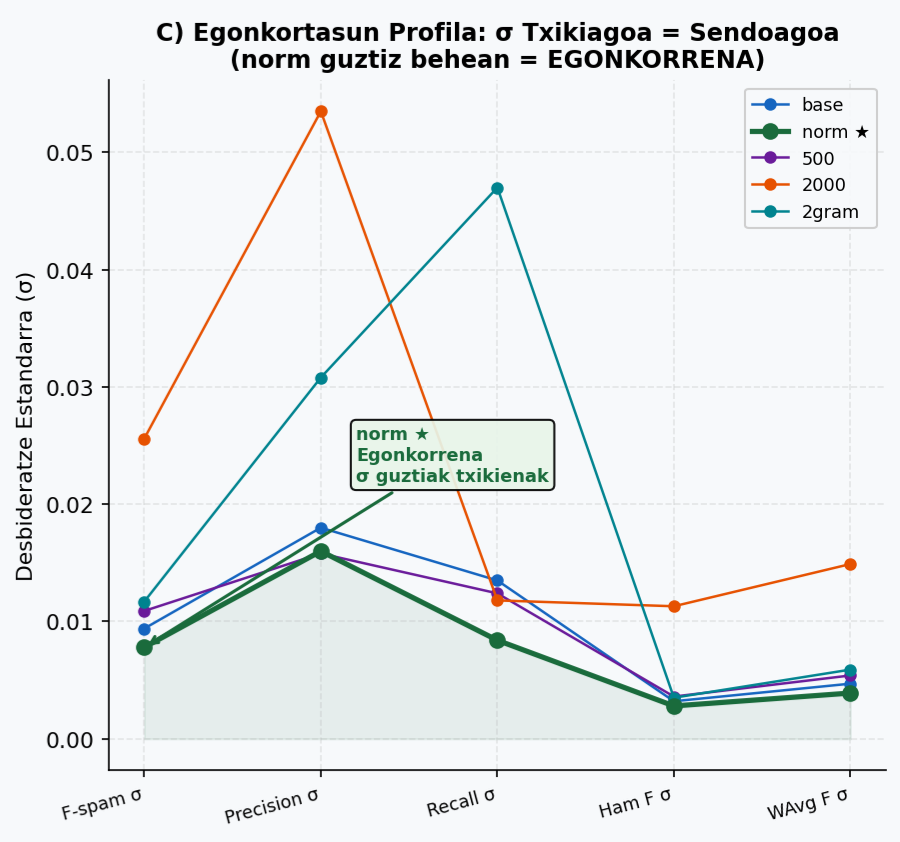
\includegraphics[width=0.9\textwidth]{diagramak/G1_metrika_konparaketa_eu_editado.PNG}
    \caption{Eredu ezberdinen sailkapen-metrika nagusien konparaketa (Spam klasea eta metrika orokorrak). Desorekatutako datuetan F-Measureak duen garrantzia nabarmentzen da.}
    \label{fig:g1_metrikak}
\end{figure}

\newpage
\subsubsection*{Ereduaren egonkortasuna eta iterazioen bilakaera}
Bigarren irudian, \textit{5 Repeated Stratified Hold-Out} ebaluazio-eskemako iterazioz iterazioko bilakaera bistaratzen da. Eredu baten benetako balioa ez datza soilik bere batezbesteko asmatze-tasan, baizik eta datu-partiketa desberdinen aurrean erakusten duen sendotasunean. Grafiko honetako lerroen gorabeherek argi erakusten dute eredu hautatuak (Norm) aldakortasun oso txikiko portaera duela iterazioetan zehar. Bariantza txiki honek bermatzen du eredua ez dela soilik datu-multzo zehatz batera gainegokitu (\textit{Overfitting}), baizik eta patroi orokorrak ikasi dituela.

\begin{figure}[H]
    \centering
    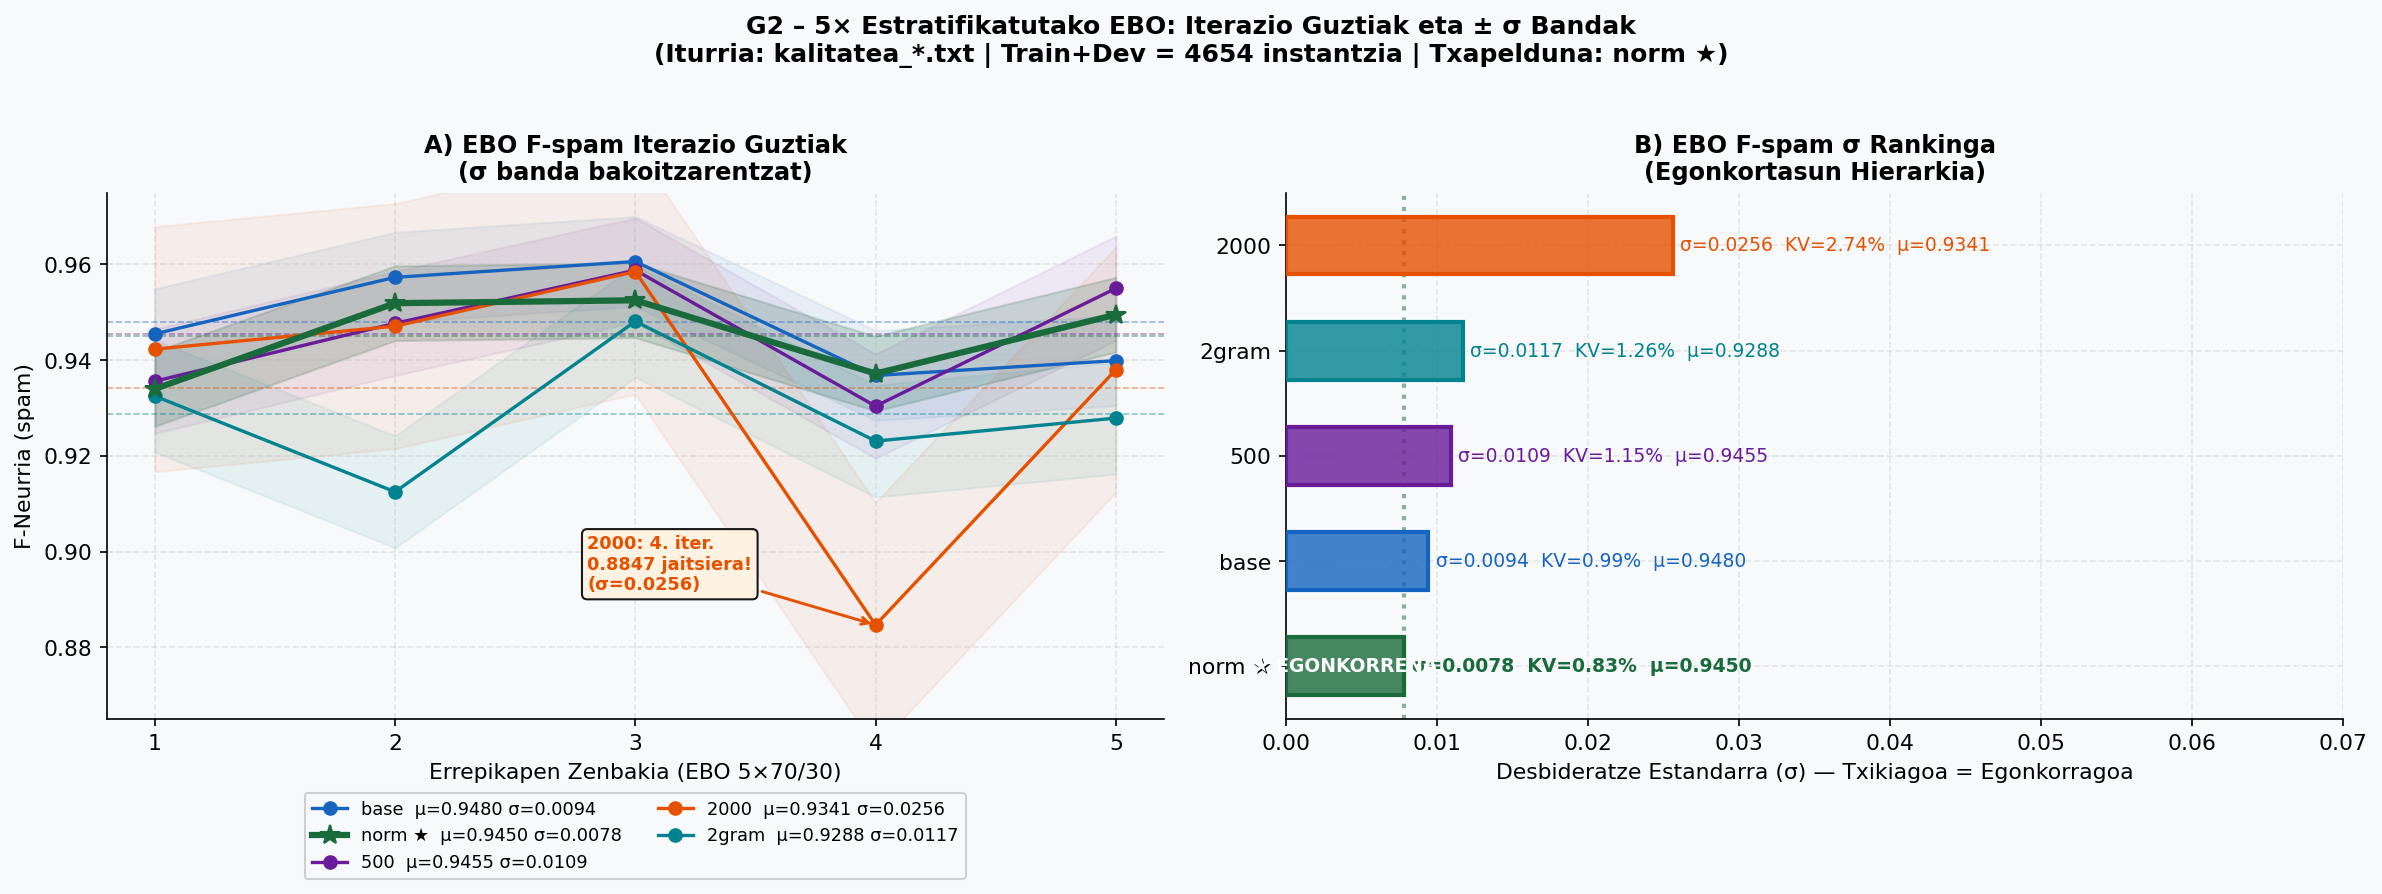
\includegraphics[width=1\textwidth]{diagramak/G2_ebo_iterazioak_eu.png}
    \caption{F-Measurearen bilakaera iterazioz iterazio. Lerroen gorabeherek datu ezezagunen aurreko egonkortasuna (edo bariantza) irudikatzen dute.}
    \label{fig:g2_iterazioak}
\end{figure}

\subsubsection*{Akatsen analisia (Konfusio-matrizeak eta inpaktu erreala)}
Sailkapen-akatsen tipologia ulertzea ezinbestekoa da posta elektronikoaren kudeaketan; izan ere, akats guztiek ez dute kostu bera. Gezurrezko Positibo batek (posta legitimo bat spam gisa ezabatzeak) erabiltzailearentzat informazio galera larria suposa dezake; Gezurrezko Negatibo batek (spam mezu bat sarrerako ontzian jasotzeak), aldiz, ez dauka inportantzia handirik. Hirugarren irudiak argi bereizten ditu errore mota hauek eredu bakoitzeko. Eredu finalak ez du soilik akats totalen kopuru optimoa mantentzen, baizik eta Gezurrezko Positiboen tasa minimizatzen laguntzen du, testuinguru erreal eta profesional baterako jarrera seguruagoa eskainiz.

\begin{figure}[H]
    \centering
    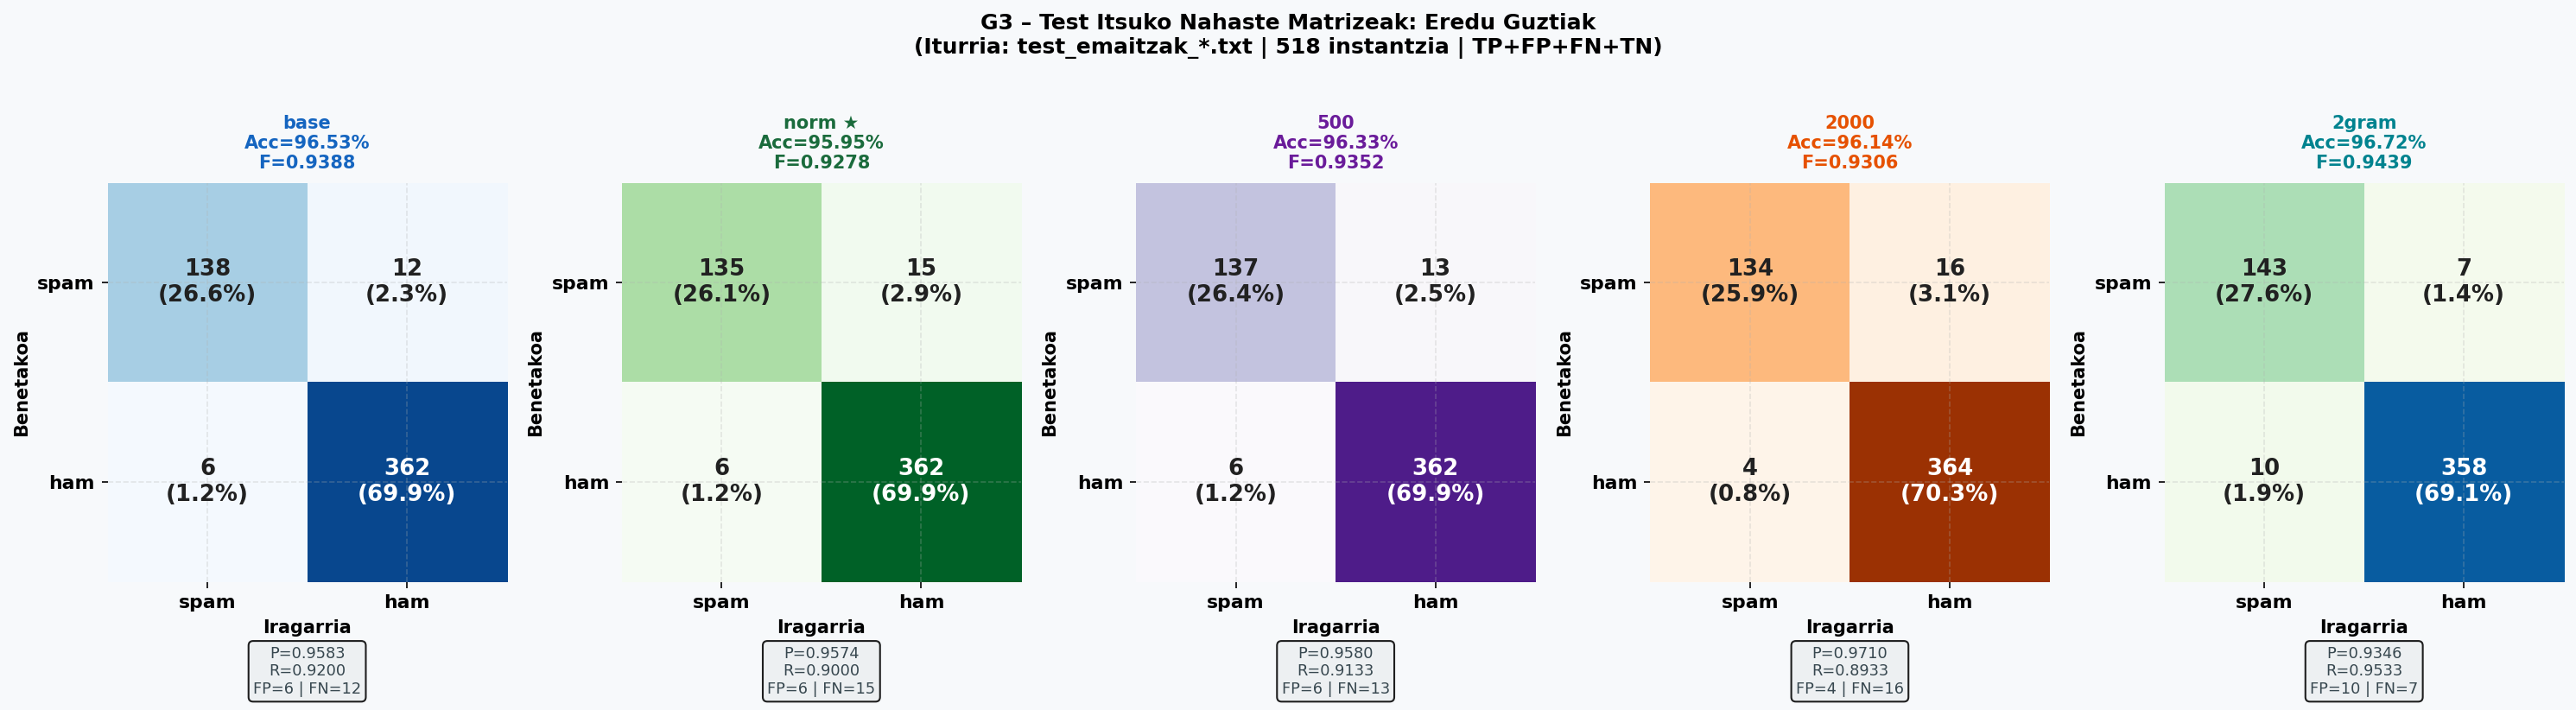
\includegraphics[width=0.9\textwidth]{diagramak/G3_nahaste_matrizeak_eu.png}
    \caption{Konfusio-matrizeen analisia: Gezurrezko Positiboen (errore kritikoagoa) eta Gezurrezko Negatiboen banaketa eredu bakoitzean.}
    \label{fig:g3_akatsak}
\end{figure}

\newpage
\subsubsection*{Erabaki multikriterioa: Errendimendu orokorra eta egonkortasuna}
Laugarren irudiko radar-diagramak argi islatzen du eredu txapelduna hautatzeko erabili den dimentsio anitzeko ikuspegia. Grafiko honek eredu bakoitzaren aztarna estatistikoa ebaluatzen du sei ardatzetan: Gurutzeko Baliozkotzeko (CV) F-Measure, Hold-Out ebaluazioko F-Measure ($\mu$), Zehaztasuna (Precision $\mu$), Estaldura (Recall $\mu$), Haztatutako batezbestekoa (WAvg F $\mu$) eta Egonkortasuna ($1-\sigma$). 

Ikus daitekeenez, erabakia ez da oinarritu metrika bakar bat maximizatzean (adibidez, CV F-spam hutsa). Aitzitik, ``Norm'' ereduak lortzen du azalera orekatuena muga guztietan, bereziki egonkortasunean (Egonk.) gailenduz. Puntuazio altuen eta bariantza txikiaren arteko oreka horrek bermatzen du eredu txapelduna dela fidagarriena ingurune erreal batean.

\subsubsection*{Errendimenduaren eta Egonkortasunaren arteko balantzea (Dispersio-grafikoa)}
Laugarren irudiaren ezkerraldeko dispersio-grafikoak EBO (Hold-Out) ebaluazioaren bi parametro kritikoenak gurutzatzen ditu: Y ardatzean Spam F-Measurearen batezbestekoa ($\mu$) eta X ardatzean desbideratze estandarra ($\sigma$). 

Machine Learning ingurune batean, eredu ideal bat grafikoaren goiko ezkerreko ertzean kokatuko litzateke (asmatze-tasa maximoa eta aldakortasun minimoa). Puntuak aztertuz gero, argi ikusten da ``Norm'' eredua dela ezkerralderago dagoena. Hau da, nahiz eta ``base'' ereduak batezbesteko apur bat altuagoa izan (Y ardatzean gorago egon), ``Norm'' ereduak bariantza askoz txikiagoa du (X ardatzean ezkerrago dago). Balantze honek erakusten du eredua gai dela datu berrien aurrean portaera iragarri bat mantentzeko, ``2000'' ereduak erakusten duen ezegonkortasunaren (eskuinalderantz lerratuta) aurrean.

\begin{figure}[H]
    \centering
    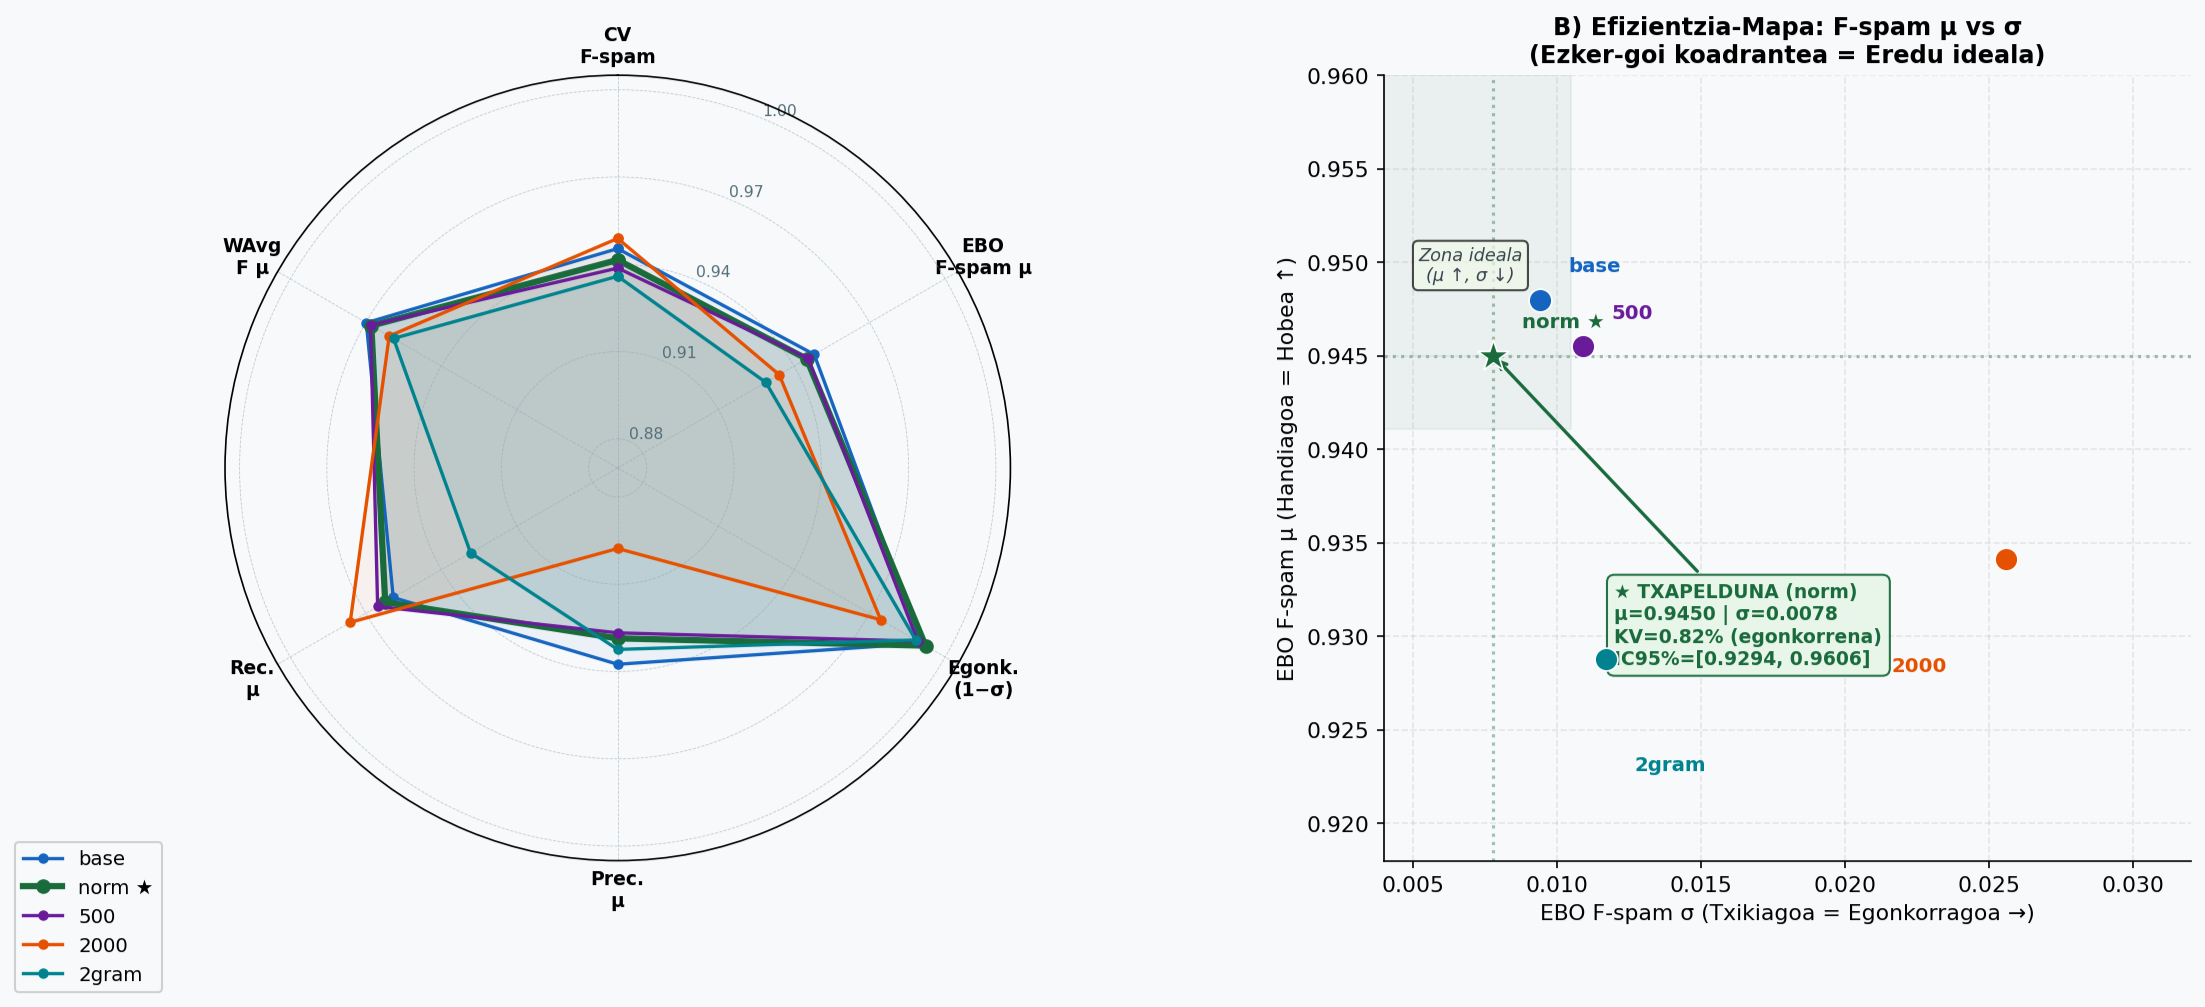
\includegraphics[width=0.9\textwidth]{diagramak/G4_radar_justifikazioa_eu_editado.PNG}
    \caption{Eredu onenaren hautaketarako analisi grafiko bikoitza: ezkerrean, errendimenduaren ($\mu$) eta egonkortasunaren ($\sigma$) arteko dispersioa; eskuinean, sei metrika estatistikoren ebaluazio multikriterioa radar-diagrama bidez.}
    \label{fig:g4_radar}
\end{figure}
\newpage
\subsubsection*{Konparaketa estatistiko zehatza: Errore-barrak}

Aurreko ataletan aipatutako egonkortasun hori maila kuantitatibo zehatzagoan aztertzeko, hurrengo grafikoan eredu bakoitzaren Spam F-Measurearen batezbestekoa ($\mu$) eta desbideratze estandarra ($\sigma$) irudikatzen dira errore-barren bitartez. 

Grafiko honek ikuspegi garbia ematen du: errore-barra zenbat eta estuagoa izan, orduan eta seguruago egon gaitezke lortuko dugun emaitzaz. Ikus daitekeen bezala, nahiz eta ``base'' ereduak batezbesteko apur bat altuagoa izan, gure eredu txapeldunak (\textbf{Norm}) du sakabanaketarik txikiena ($\sigma=0{,}0078$). Horrek esan nahi du eredu horrek portaera askoz aurreikusgarriagoa duela diseinutik kanpoko egoeretan, ``2000'' bezalako eredu konplexuago batek erakusten duen ziurgabetasun altuaren ($\sigma=0{,}0256$) aldean.

\begin{figure}[H]
\centering
\begin{tikzpicture}
\begin{axis}[
    title={\textbf{Hold-Out F-Measure eta Desbideratze Estandarra}},
    width=12cm,
    height=8cm,
    ylabel={Spam F-Measure (batezbestekoa $\pm\,\sigma$)},
    xlabel={Ebaluatutako Eredua},
    % Identifikatzaile barneko seguruak
    symbolic x coords={C1, C2, C3, C4, C5},
    xtick=data,
    % Ardatzean erakutsiko diren benetako etiketak
    xticklabels={Norm (Txapelduna), 2000, 2Gram, 500, base},
    x tick label style={font=\small},
    ymin=0.890,
    ymax=0.985, 
    ymajorgrids=true,
    grid style=dashed,
    legend style={at={(0.97,0.03)}, anchor=south east, font=\small}, 
    error bars/y dir=both,
    error bars/y explicit,
    error bars/error bar style={thick, black},
    error bars/error mark options={rotate=90, mark size=4pt, black, thick},
    mark size=5pt,
]

% Datuen irudikapena
\addplot[
    only marks,
    mark=*,
    mark options={fill=orange!80, draw=orange!90!black}
] 
coordinates {
    (C1, 0.9450) +- (0, 0.0078)
    (C2, 0.9341) +- (0, 0.0256)
    (C3, 0.9288) +- (0, 0.0117)
    (C4, 0.9455) +- (0, 0.0109)
    (C5, 0.9480) +- (0, 0.0094)
};
\addlegendentry{Hold-Out F-Measure ($\pm\,\sigma$)}

% Desbideratze estandarraren balioak errore-barren gainean idatzita
\node[font=\small, blue!70!black, above, yshift=5pt] at (axis cs:C1, 0.9528) {$\sigma\!=\!0{,}0078$};
\node[font=\small, red!70!black, above, yshift=5pt] at (axis cs:C2, 0.9597) {$\sigma\!=\!0{,}0256$};
\node[font=\small, black!60, above, yshift=5pt] at (axis cs:C3, 0.9405) {$\sigma\!=\!0{,}0117$};
\node[font=\small, black!60, above, yshift=5pt] at (axis cs:C4, 0.9564) {$\sigma\!=\!0{,}0109$};
\node[font=\small, black!60, above, yshift=5pt] at (axis cs:C5, 0.9574) {$\sigma\!=\!0{,}0094$};

% Eredu txapeldunaren erreferentzia lerroa
\draw[dotted, blue!60!black, thick]
    (axis cs:C1, 0.9450) -- (axis cs:C5, 0.9450)
    node[pos=1, above left, font=\tiny] {Norm: $\mu=0{,}9450$};

\end{axis}
\end{tikzpicture}
\caption{Spam klaseko F-Measurearen batezbestekoa eta desbideratze estandarra ($\sigma$). Errore-barren tamaina estuak egonkortasuna bermatzen du. \textbf{Norm} ereduak du sakabanaketa estatistiko txikiena ($\sigma=0{,}0078$).}
\label{fig:errore_barrak_fmeasure}
\end{figure}
\newpage
% =============================================
% 6. KALITATE ESTIMATUA
% =============================================
\section{Aurreikusitako kalitate estimatua}

Atal honetan ebaluatutako bost ereduen (\textit{Oinarrizkoa}, \textit{2000 atributukoa}, \textit{500 atributukoa}, \textit{2-gram} eta \textit{Normalizatua}) kalitate estimatua aztertuko da, \textbf{train eta dev instantziak elkartuz} (guztira 4.654 instantzia). Ebaluazioa egiteko bi eskema erabili dira: 5-fold Cross Validation eta 5 Repeated Stratified Hold-Out (70/30).

\subsection{Ereduen arteko konparaketa eta azterketa}

Eredu bakoitzaren fidagarritasuna eta egonkortasuna neurtzeko, bi ebaluazio-eskemekin lortutako emaitza nagusiak alderatuko ditugu.

Hona hemen 5-fold Cross Validation bidez lortutako metrika nagusiak bost ereduetarako:

\begin{table}[H]
    \centering
    \caption{Bost ereduen 5-fold Cross Validation emaitzen konparaketa}
    \begin{tabular}{lcccc}
        \toprule
        \textbf{Eredua} & \textbf{Accuracy} & \textbf{Spam F-Measure} & \textbf{Ham F-Measure} & \textbf{WAvg F-Measure} \\
        \midrule
        Oinarrizkoa   & \%96,82 & 0,9454 & 0,9776 & 0,9682 \\
        2000 atributu & \%97,03 & 0,9489 & 0,9791 & 0,9704 \\
        500 atributu  & \%96,43 & 0,9387 & 0,9748 & 0,9644 \\
        2-gram        & \%96,28 & 0,9359 & 0,9738 & 0,9628 \\
        Normalizatua  & \%96,61 & 0,9415 & 0,9761 & 0,9661 \\
        \bottomrule
    \end{tabular}
\end{table}

Ikusten denez, 5-fold CV bidez, \textit{2000 atributuko} eredua da zehaztasun handiena lortzen duena (Accuracy \%97,03 eta Spam F-Measure 0,9489), eta atzetik oinarrizko eredua dago. \textit{Normalizatutako} eredua hirugarren postuan geratzen da, oso emaitza lehiakorrak lortuz baina ez altuenak.

Hala ere, eredu baten fidagarritasun erreala neurtzeko ezinbestekoa da bere egonkortasuna aztertzea; izan ere, kasu guztietan zehaztasuna hain handia denean, hobe izaten da desbideratze estandarra minimizatzen duen eredua aukeratzea, zehaztasuna maximizatzen duena baino. Horretarako, 5 Repeated Stratified Hold-Out (70/30) emaitzak eta haien desbideratze estandarrak ($\pm$) alderatuko ditugu:

\begin{table}[H]
    \centering
    \caption{Bost ereduen 5 Repeated Stratified Hold-Out (70/30) emaitzen konparaketa}
    \resizebox{\textwidth}{!}{%
    \begin{tabular}{lccc}
        \toprule
        \textbf{Eredua} & \textbf{Spam F-Measure} & \textbf{Ham F-Measure} & \textbf{WAvg F-Measure} \\
        \midrule
        Oinarrizkoa   & $0{,}9480 \pm 0{,}0094$ & $0{,}9786 \pm 0{,}0032$ & $0{,}9698 \pm 0{,}0047$ \\
        2000 atributu & $0{,}9341 \pm 0{,}0256$ & $0{,}9713 \pm 0{,}0113$ & $0{,}9607 \pm 0{,}0149$ \\
        500 atributu  & $0{,}9455 \pm 0{,}0109$ & $0{,}9773 \pm 0{,}0036$ & $0{,}9681 \pm 0{,}0054$ \\
        2-gram        & $0{,}9288 \pm 0{,}0117$ & $0{,}9712 \pm 0{,}0035$ & $0{,}9590 \pm 0{,}0059$ \\
        Normalizatua  & $0{,}9450 \pm 0{,}0078$ & $0{,}9771 \pm 0{,}0028$ & $0{,}9678 \pm 0{,}0039$ \\
        \bottomrule
    \end{tabular}%
    }
\end{table}

\subsection{Eredu finalaren hautaketa}

Emaitza hauek aztertuta, \textbf{Normalizatutako eredua} hautatu dugu azken eredu gisa. Nahiz eta 5-fold CV bidez lortutako zehaztasun handienak beste eredu batzuek lortu dituzten (adibidez, 2000 atributukoak), aldea oso txikia da (Normalizatutakoaren eta 2000 atributukoaren arteko diferentzia F-Measure Spam metrikan 0,0074koa baino ez da).

Hala ere, Repeated Hold-Out ebaluazioak argi erakusten du Normalizatutako eredua dela denetan \textbf{egonkorrena}, desbideratze estandar txikienak aurkezten baititu metrika guztietan:
\begin{itemize}
    \item Spam F-Measure: $\pm 0{,}0078$
    \item Ham F-Measure: $\pm 0{,}0028$
    \item WAvg F-Measure: $\pm 0{,}0039$
\end{itemize}

Desbideratze txiki hauek bermatzen dute ereduak ez duela gehiegizko doikuntzarik (overfitting) eta portaera sendoa eta errepikagarria izango duela datu berrien aurrean. Hori dela eta, zehaztasun maximoa gutxigatik sakrifikatu dugu egonkortasun handiagoaren truke.

\subsection{Filtro konbinaketak}

Oinarrizko prozeduraz gain, filtro konbinaketa gehiago ere probatu dira proiektu honetan. Proba guztiek ondorio berberetara eramaten gaituzten arren, bi konbinazio hauek aukeratu dira eredu adierazgarri gisa: testuen normalizazioa bigramekin (2-gram) batera, eta normalizazioa maiztasun-atalasearekin (\textit{threshold}) batera.

\begin{table}[htbp]
\centering
    \caption{Filtro konbinaketen bidezko emaitzen batezbestekoa eta desbideratze estandarra.}
\label{tab:filtro_konbinaketak}
\begin{tabular}{lcccc}
\hline
\textbf{Konfigurazioa} & \textbf{Precision} & \textbf{Recall} & \textbf{F-Measure} & \textbf{WAvg F-Meas.} \\ \hline
Norm + 2gram & $0{,}9210 \pm 0{,}0478$ & $0{,}9378 \pm 0{,}0471$ & $0{,}9272 \pm 0{,}0183$ & $0{,}9576 \pm 0{,}0102$ \\
Norm + Thresh. & $0{,}9218 \pm 0{,}0229$ & $0{,}9416 \pm 0{,}0385$ & $0{,}9306 \pm 0{,}0097$ & $0{,}9596 \pm 0{,}0046$ \\ \hline
\end{tabular}
\end{table}

\noindent
Taulan ikus daitekeenez, batez ere \textit{Norm + 2gram} kasuan, desbideratze estandarra altuagoa da. Gainera, filtroak konbinatzeak entrenamendu denborak luzatzea ekarri du kasu askotan (200 segundotik gora zenbait kasutan), lortutako etekin eskasari begira merezi ez duen karga kalkulatzailea erantsiz. Beraz, eredu hauek baztertu egin dira, beste konfigurazio orekatuagoen eta sinpleagoen alde egiteko.

\subsection{Hautatutako ereduaren ebaluazio aurreratua}

Eredu normalizatuaren parametro optimoak honako hauek dira:
\begin{itemize}
    \item LearningRate: 0,01
    \item Momentum: 0,1
    \item HiddenLayers: 3
    \item Epochs: 500
\end{itemize}

\subsubsection*{5-fold Cross Validation}

\begin{table}[H]
    \centering
    \caption{Normalizatutako ereduaren 5-fold CV emaitzak}
    \begin{tabular}{lrrr}
        \toprule
        \textbf{Klasea} & \textbf{Precision} & \textbf{Recall} & \textbf{F-Measure} \\
        \midrule
        Spam  & 0,9408 & 0,9422 & 0,9415 \\
        Ham   & 0,9764 & 0,9758 & 0,9761 \\
        WAvg  & 0,9661 & 0,9661 & 0,9661 \\
        \midrule
        \multicolumn{2}{l}{Accuracy} & \multicolumn{2}{r}{\%96,61} \\
        \bottomrule
    \end{tabular}
\end{table}

Nahaste-matrizea:

\begin{table}[H]
    \centering
    \caption{Normalizatutako ereduaren 5-fold CV nahaste-matrizea}
    \begin{tabular}{rr|l}
        \toprule
        \textbf{a} & \textbf{b} & \\
        \midrule
        1272 & 78  & a = spam \\
        80   & 3224 & b = ham  \\
        \bottomrule
    \end{tabular}
\end{table}

\subsubsection*{5 Repeated Stratified Hold-Out (70/30)}

\begin{table}[H]
    \centering
    \caption{Repeated Hold-Out emaitzak iterazioz iterazio (Normalizatua)}
    \begin{tabular}{lrrr}
        \toprule
        \textbf{Iterazioa} & \textbf{F-spam} & \textbf{F-ham} & \textbf{WAvg-F} \\
        \midrule
        1 & 0,9340 & 0,9720 & 0,9611 \\
        2 & 0,9519 & 0,9789 & 0,9708 \\
        3 & 0,9525 & 0,9795 & 0,9714 \\
        4 & 0,9372 & 0,9764 & 0,9658 \\
        5 & 0,9495 & 0,9786 & 0,9701 \\
        \bottomrule
    \end{tabular}
\end{table}

\begin{table}[H]
    \centering
    \caption{Repeated Hold-Out batezbestekoa $\pm$ desbideratze estandarra (Normalizatua)}
    \begin{tabular}{lrrr}
        \toprule
        \textbf{Klasea} & \textbf{Precision} & \textbf{Recall} & \textbf{F-Measure} \\
        \midrule
        Spam & $0{,}9286 \pm 0{,}0160$ & $0{,}9623 \pm 0{,}0084$ & $0{,}9450 \pm 0{,}0078$ \\
        Ham  & $0{,}9845 \pm 0{,}0027$ & $0{,}9698 \pm 0{,}0071$ & $0{,}9771 \pm 0{,}0028$ \\
        WAvg & --                       & --                       & $0{,}9678 \pm 0{,}0039$ \\
        \bottomrule
    \end{tabular}
\end{table}

Emaitzek erakusten dute aukeratutako ereduak portaera sendoa duela bi klaseetan, desbideratze estandar txikiekin, datu ezezagunen aurrean orokortze ona bermatuz.

\newpage
% =============================================
% 7. IRAGARPENAK -- ERABILTZAILE PAKETEA
% =============================================
\section{Erabiltzailearen paketea}

\subsection{Paketearen edukia eta helburua}

Erabiltzaileari entregatzen zaion paketeak testu gordina sartu eta spam/ham 
iragarpenak lortzeko behar den guztia biltzen du:

\begin{itemize}
    \item \textbf{Eredu entrenatua}: \texttt{modelo/mlp.model} (MultilayerPerceptron)
    \begin{itemize}
            \item Instantzia guztiekin entrenatutakoa.
        \end{itemize}
    \item \textbf{Ereduaren ebaluaketa}: \texttt{test\_emaitzak\_norm.txt}, \texttt{kalitatea\_norm.txt}
    \item \textbf{Aurreprozesamenduko filtroak}:
    \begin{itemize}
        \item \texttt{modelo/normalizer.ser}
        \begin{itemize}
            \item Fitxategi hau TextNormalizer filtroa erabili dela adierazteko da.
            \item Eredu optimoak beti izango du, baina erabaki dugu fitxategi hau mantentzea kode orokorrago bat izateko.
        \end{itemize}
        \item \texttt{modelo/vectorizer.ser} (StringToWordVector, TF-IDF)
        \item \texttt{modelo/selector.ser} (AttributeSelection, InfoGain)
    \end{itemize}
    \item \textbf{Inferentzia klasea}: \texttt{Iragarri.java}
    \item \textbf{Utilities klaseak}: \texttt{FilterSerializationHelper.java}, \texttt{TextNormalizer.java}
    \item \textbf{Weka liburutegia}: \texttt{lib/weka.jar}
    \item \textbf{Dokumentazioa}: Javadoc eta erabilera eskuliburua
\end{itemize}

\subsection{Inferentzia pipeline-a: Iragarri.java}

\texttt{Iragarri.java} klaseak sarrerako direktorio batean dauden \texttt{.txt} fitxategiak (mezu elektroniko gordinak) kargatzen ditu eta bakoitzari dagokion \textit{spam}/\textit{ham} iragarpena egiten dio. Prozesuak entrenamenduko pipeline osoa errepikatzen du koherentzia bermatzeko:

\begin{enumerate}
    \item \textbf{Karga}: \texttt{.txt} fitxategiak direktorio lautik kargatu eta \texttt{Instances} objektu bilakatu, klase ezezagunarekin.
    \item \textbf{Normalizazioa}: \texttt{normalizer.ser} existitzen bada, TextNormalizer aplikatu (URLak, emailak, HTML garbitu).
    \item \textbf{Bektorizazioa}: \texttt{vectorizer.ser} kargatu eta aplikatu (TF-IDF, tokenizazioa, stemming, stopwords).
    \item \textbf{Atributu-hautaketa}: \texttt{selector.ser} aplikatu, InfoGain bidez hautatutako atributuak mantentzeko.
    \item \textbf{Sailkapena}: Eredua kargatu eta \texttt{classifyInstance()} + \texttt{distributionForInstance()} bidez iragarpenak eta konfidantza-mailak kalkulatu.
    \item \textbf{Emaitzak gorde}: \texttt{iragarpenak.txt} fitxategian iragarpenak erregistratu.
\end{enumerate}

\subsubsection*{Exekuzio adibidea}

\begin{verbatim}
java --add-opens java.base/java.lang=ALL-UNNAMED \
     -cp "lib/weka.jar:bin" Iragarri \
     modelo/mlp.model data_proba/ iragarpenak/
\end{verbatim}

Irteera kontsolan eta \texttt{emaitzak/iragarpenak.txt} fitxategian:

\begin{verbatim}
==================================================
               IRAGARPENAK - EMAITZAK             
==================================================

1. mezua: SPAM (zehaztasuna: 0.9939)
2. mezua: HAM (zehaztasuna: 0.9993)
3. mezua: HAM (zehaztasuna: 0.5998)
4. mezua: SPAM (zehaztasuna: 0.9939)

==================================================
Guztira sailkatutako mezuak: 4
==================================================
\end{verbatim}

\subsection{Ereduaren muga funtzionalak: hizkuntza-mendekotasuna}

Eredua ingelesezko emailekin entrenatu denez, hizkuntza horretarako optimizatuta dago. Hau frogatzeko, 12 mezu berri probatu ditugu hiru hizkuntzatan (ingelesa, gaztelania eta euskara), 2 spam eta 2 ham hizkuntza bakoitzeko:

\begin{table}[H]
    \centering
    \caption{Iragarpenak hizkuntza desberdinetan}
    \begin{tabular}{llll}
        \toprule
        \textbf{Hizkuntza} & \textbf{Mota} & \textbf{Iragarpena} & \textbf{Zuzena?} \\
        \midrule
        Ingelesa & Ham  & HAM (0,9268)  & \ding{51} \\
        Ingelesa & Ham  & HAM (0,9938)  & \ding{51} \\
        Ingelesa & Spam & SPAM (0,9993) & \ding{51} \\
        Ingelesa & Spam & SPAM (0,9986) & \ding{51} \\
        \midrule
        Gaztelania & Ham  & SPAM (0,9743)  & \ding{55} \\
        Gaztelania & Ham  & SPAM (0,9095) & \ding{55} \\
        Gaztelania & Spam & SPAM (0,9335)  & \ding{51} \\
        Gaztelania & Spam & HAM (0,5469)  & \ding{55} \\
        \midrule
        Euskara & Ham  & HAM (0,9943)  & \ding{51} \\
        Euskara & Ham  & HAM (0,5365)  & \ding{51} \\
        Euskara & Spam & SPAM (0,8892)  & \ding{55} \\
        Euskara & Spam & HAM (0,5998)  & \ding{51} \\
        \bottomrule
    \end{tabular}
    \label{tab:lang_test}
\end{table}

\begin{itemize}
    \item \textbf{Ingelesa}: 4/4 zuzen (\%100 accuracy), konfidantza-maila 
          altuekin (0,97-0,99).
    \item \textbf{Gaztelania}: 1/4 zuzen (\%25). Spam gisa sailkatzeko joera, konfidantza-maila altuarekin.
    \item \textbf{Euskara}: 3/4 zuzen (\%75), baina horietako bi konfidantza-maila baxuarekin.
\end{itemize}

Emaitza hauek ikusita, argia da ereduak ingelesez soilik dela fidagarria. Izan ere, hizkuntza desberdinetan antzeko hitzak egon daitezken arren, hau ez da gehiengo kasua izango, mezuaren testuinguru eta informazio gehiena galduz; gure euskarazko proba kasuetako bat, hain zuzen ere, atributurik gabe geratu da bektorizazioaren ondoren, klase ezezaguna soilik edukiz.

Ingesez ez diren mezuak sailkatzeko hobe izango da beste eredu bat erabiltzea, hizkuntza horretarako bereziki prestatua edota eleaniztuna.

\subsection{Kalitate-egiaztapena}
Paketearen fidagarritasuna bermatzeko, bi ebaluazio-txosten entregatzen dira:

\subsubsection{Blind Test}

\texttt{test\_emaitzak\_norm.txt} fitxategiak ereduaren errendimendu erreala erakusten du datu ezezagunen gainean. Test multzoak 517 instantzia ditu, entrenamenduan inoiz ikusi ez direnak:

\begin{table}[H]
    \centering
    \caption{Test multzoko emaitzak (ebaluazio itsua)}
    \begin{tabular}{lr}
        \toprule
        \textbf{Metrika} & \textbf{Balioa} \\
        \midrule
        Accuracy                    & \%95,95 \\
        F-Measure haztatua (WAvg)   & 0,9591  \\
        \midrule
        Spam Precision              & 0,9574  \\
        Spam Recall                 & 0,9000  \\
        Spam F-Measure              & 0,9278  \\
        \bottomrule
    \end{tabular}
    \label{tab:test_blind}
\end{table}

\begin{table}[H]
    \centering
    \caption{Test multzoko nahaste-matrizea}
    \begin{tabular}{rr|l}
        \toprule
        \textbf{a} & \textbf{b} & \\
        \midrule
        135 & 15 & a = spam \\
        6  & 362 & b = ham \\
        \bottomrule
    \end{tabular}
    \label{tab:test_confusion_blind}
\end{table}

Emaitza hauek benetako erabilera-baldintzetan espero daitekeen errendimendua islatzen dute, datu ezezagunen gaineko ebaluazio itsua delako. Bezeroak, asko jota, emaitza hobeak lortuko ditu, berak jasoko duen eredua instantzia guztiekin entrenatutakoa izango da eta.

\subsubsection{Kalitate-estimazio sendoa}

\texttt{kalitatea\_norm.txt} fitxategiak, 6.4 atalean azaldu dugun bezala, ereduaren egonkortasuna eta fidagarritasuna erakusten du bi ebaluazio-eskema independente erabiliz: 5-fold Cross Validation eta 5 Repeated Stratified Hold-Out (70/30). Ebaluazio honen emaitzak ikusteko, zoaz \textit{6.4. Hautatutako ereduaren ebaluazio aurreratua} atalera.

\newpage
% =============================================
% 8. SOFTWARE DISEINUA
% =============================================
\section{Diseinua}

Helburuetan bi rol bereizten dira: datuen pre-prozesamendua eta ebaluazioa. Atal bakoitzerako diseinatu dugun softwarearen diseinua grafikoan adierazten da datuen fluxu-diagramen bitartez, non prozesu nagusiak eta datuen transformazioak ikus daitezkeen.

\subsection{Datu-fluxu diagrama}

\begin{figure}[h!]
    \centering
     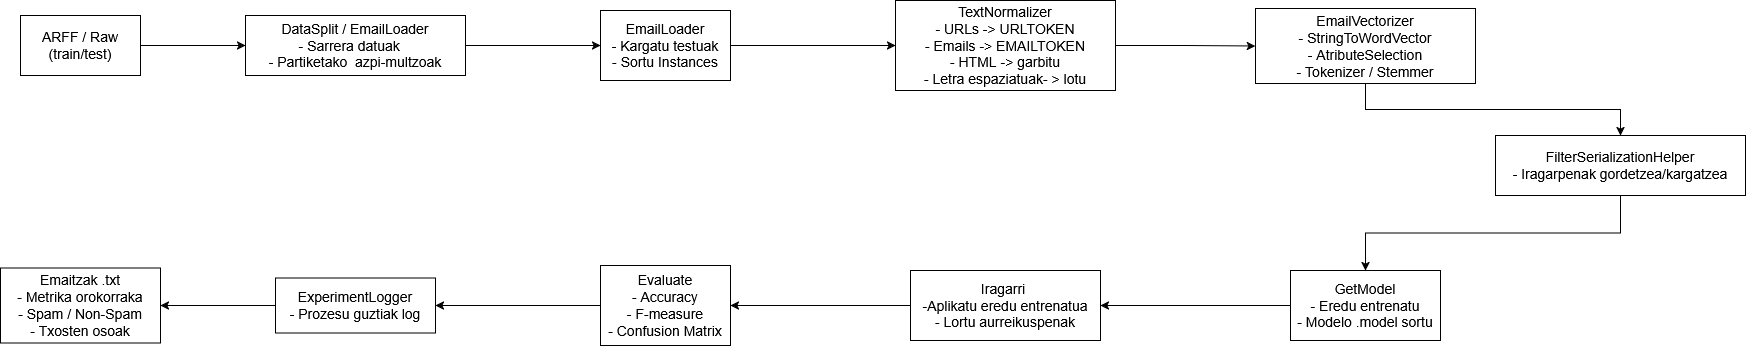
\includegraphics[width=1.17\textwidth]{diagramak/fuxu_diagrama.drawio.png}
    \caption{Datu-fluxu sinplea: sarrera, prozesuak eta irteerak.}
\end{figure}

Lehenik, sarrerako datuak (\texttt{EmailLoader} eta \texttt{DataSplit} bidez) kargatzen eta
partiketan banatzen dira. Ondoren, \texttt{TextNormalizer} osagaiak testuak garbitzen ditu URLak, helbide elektronikoak eta HTML etiketak normalizatzeta \texttt{EmailVectorizer}
osagaiak testu garbituak zenbakizko bektore bihurtzen ditu, TF-IDF, Stemming eta AttributeSelection teknikak erabiliz. \texttt{FilterSerializationHelper} osagaiak bektorizazio
prozesua gordetzen du, test multzoarekin bateragarritasuna bermatzeko.

Ondoren, \texttt{GetModel} osagaiak MLP sailkatzailearen parametro ekorketa egiten du
train eta dev multzoak erabiliz, eta modelo optimoa \texttt{.model} formatuan gordetzen du.
Ondoren, \texttt{Iragarri} osagaiak modelo hori kargatzen du eta testu berrien gainean
iragarpenak egiten ditu.

Azkenik, \texttt{Evaluate} osagaiak modeloaren kalitatea neurtzen du accuracy, F-measure eta
confusion matrix bezalako metrikak erabiliz, eta \texttt{ExperimentLogger} osagaiak prozesu
guztien parametroak eta emaitzak automatikoki erregistratzen ditu. Emaitza guztiak \texttt{.txt}
fitxategi batean gordetzen dira, txosten oso bat osatuz.

\subsection{Klase-diagrama}

\begin{figure}[H]
    \centering
    \includesvg[width=0.84\textwidth]{diagramak/KlaseDiagrama.svg}
    \caption{Proiektuaren klase-diagrama nagusia, Java fitxategien arteko erlazioak eta dependentziak erakusten dituena.}
    \label{fig:klase-diagrama}
\end{figure}
Gure softwareak 10 Java fitxategik osatzen dute: 3 datuen pre-prozesamendurako (irudian berdez agertzen direnak), 4 ereduaren entrenamendu eta ebaluazioentzat (irudian laranjaz edo urdinez agertzen direnak), eta beste 3 klase lagungarri gisa (irudian morez), exekuzio-fluxu nagusiaren parte ez diren arren, beste klaseek erabiltzen dituztenak.

Hainbat klasek funtzio publikoak dituzte, beste klaseetatik deitzen direnak. Hortaz, fitxategien artean dependentzia erlazio bat sortzen da, \texttt{EmailLoader.java} eta \texttt{ExperimentLogger.java} izanik klase dependente gehien dituzten klaseak.


\subsection{Sarrera eta Irteerak}

\begin{itemize}
    \item \textbf{Sarrera:} ARFF formatuko fitxategiak, adibidez, \texttt{test\_final.arff} edo \texttt{train\_final.arff}, partiketako azpi-multzoak erabiliz.
    \item \textbf{Barneko prozesuak:}
    \begin{itemize}
        \item \textbf{Pre-prozesamendua:} testu normalizazioa (\texttt{TextNormalizer}), tokenizazioa eta atributuen selekzioa (\texttt{StringToWordVector}, \texttt{AttributeSelection}).
        \item \textbf{Inferentzia:} entrenatutako ereduak aplikatzea (\texttt{Classifier} erabiltzen \texttt{Iragarri} eta \texttt{TestModel} klaseetan).
        \item \textbf{Ebaluazioa:} zehaztasuna, recall eta F-measure kalkulatzea (\texttt{Evaluation} klasearen bidez).
    \end{itemize}
    \item \textbf{Irteera:} testuen emaitzak fitxategi testuetan gordetzea (\texttt{.txt}), baita konfusio-matrizeak eta metrika orokorrak.
\end{itemize}

\subsection{Datuen transformazioa}

Datuak sarreratik irteerara prozesu hauen bidez pasatzen dira:

\begin{enumerate}
    \item Sarrerako ARFF fitxategia kargatu eta datu-egitura prestatu (\texttt{EmailLoader}).
    
    \item Testu atributuak normalizatu aurreprozesamendu gisa, zarata murrizteko (\texttt{TextNormalizer}).
    
    \item Testua bektore bihurtu eta atributu esanguratsuenak hautatu
    (\texttt{StringToWordVector}, \texttt{AttributeSelection}).
    
    \item Entrenatutako ereduarekin inferentzia aplikatu,
    instantzia bakoitza sailkatzeko (\texttt{Classifier}).
    
    \item Emaitzak ebaluatu metrika estandarren bidez eta txostenak sortu
    (\texttt{Evaluation}, \texttt{.txt} fitxategiak).
\end{enumerate}

Horrela, datuen fluxua eta prozesu nagusiak modu grafiko eta testualean dokumentatzen dira, sarrera eta irteera formatuak argi adieraziz.

% =============================================
% X. ADIMEN ARTIFIZIALAREN ERABILERA
% =============================================
\newpage
\section{Adimen Artifizialaren erabilera}

Proiektu honen garapenean, Adimen Artifizial sortzaileko tresnak (hala nola, Claude edo Gemini) erabili dira laguntzaile tekniko gisa, betiere, hauek emandako erantzunen errepasoa bermatzen.Tresna hauek garapen-prozesua arintzeko eta azken entregagarrien kalitate formala hobetzeko erabili dira.

Zehazki, honako zeregin hauetarako erabili da IA tresnen laguntza:

\begin{itemize}
    \item \textbf{Dokumentazioaren berrikuspena eta estilo-zuzenketa:} Txosteneko hainbat ataletan, testuen koherentzia, gramatika eta tonu akademikoa hobetzeko erabili da. Ideiak, argudioak eta ondorioak behin garatuta IA erabili da esaldiak hobeto egituratzeko eta irakurgarritasuna bermatzeko.
    \item \textbf{Estetika eta LaTeX formatua:} Txostena idazteko orduan, LaTeX formatuko taula konplexuen, ekuazioen eta irudien sintaxia doitzeko laguntza eskatu da, maketazio-denbora aurreztuz.
    \item \textbf{Zeregin errepikakorren programazioa:} Kodearen egitura orokorrak, salbuespenen kudeaketa (\textit{try-catch} blokeak) edo fitxategiak irakurri/idazteko oinarrizko egiturak azkarrago garatzeko erabili da, taldeak logika nagusian zentratu ahal izateko.
    \item \textbf{Weka liburutegiaren ikerketa:} Wekako klaseen eta API-aren dokumentazio ofizial zabala azkarrago arakatzeko eta klase jakin batzuen (adibidez, \texttt{StringToWordVector} edo \texttt{MultilayerPerceptron}) parametroen funtzionamendua argitzeko bilatzaile aurreratu gisa erabili da.
    \item \textbf{Kodearen dokumentazioa (JavaDoc):} Klaseen eta metodoen goiburuetako JavaDoc iruzkin estandarrak (\texttt{@param}, \texttt{@return}) era erdi-automatikoan sortzeko laguntzaile gisa erabili da, kodea ulergarriagoa eta garbiagoa izan dadin.
\end{itemize}

Laburbilduz, Adimen Artifizialaren erabilera proiektuaren kalitate formala eta garapen-abiadura hobetzeko baliabide osagarri gisa erabili da. Tresna hauek iradokitako testu, kode-egitura edo soluzio guztiak arretaz berrikusi, balioztatu eta proiektuaren behar espezifikoetara egokitu dira, emaitza finala taldearen irizpide teknikoen eta ezagutzaren isla fidela izan dadin.

% =============================================
% BIBLIOGRAFIA
% =============================================
\newpage
\bibliographystyle{plain}
\begin{thebibliography}{9}

\bibitem{goodfellow2016}
Goodfellow, I., Bengio, Y., \& Courville, A. (2016).
\textit{Deep Learning}. MIT Press.

\bibitem{bishop2006}
Bishop, C. M. (2006).
\textit{Pattern Recognition and Machine Learning}. Springer.

\bibitem{weka}
Hall, M., Frank, E., Holmes, G., Pfahringer, B., Reutemann, P., \& Witten, I. H. (2009).
The WEKA data mining software: An update.
\textit{ACM SIGKDD Explorations Newsletter}, 11(1), 10--18.

\bibitem{manning}
Manning, C. D., Raghavan, P., \& Sch\"utze, H. (2008).
\textit{Introduction to Information Retrieval}. Cambridge University Press.

\bibitem{hastie}
Hastie, T., Tibshirani, R., \& Friedman, J. (2009).
\textit{The Elements of Statistical Learning}. Springer.

\bibitem{alpaydin2010}
Alpaydin, E. (2010).
\textit{Introduction to Machine Learning} (2nd ed.). MIT Press.

\bibitem{wekamanual2011}
Bouckaert, R. R., Frank, E., Hall, M., Kirkby, R., Reutemann, P., Seewald, A., \& Scuse, D. (2011).
\textit{WEKA Manual for Version 3-6-6}. University of Waikato, Hamilton, New Zealand.

\end{thebibliography}



\end{thebibliography}

\end{document}